\section*{Motivation}
A classical application of modular forms is to find equalities of arithmetical functions,
by finding modular forms whose Fourier coefficients are those arithmetical functions, and then
finding identities of modular forms which follow from dimensional considerations. Our goal for
this session will be to prove the following well know identities:

\begin{align*}
    \sigma_7(n) &= \sigma_3(n)+\sum_{i=1}^{n-1}\sigma_3(i)\sigma_3(n-1) \\
    11\sigma_9(n) &= 21\sigma_5(n)-10\sigma_3(n)+5040\sum_{i=1}^{n-1}\sigma_3(i)\sigma_5(n-1) \\
    \sigma_{13}(n) &= 21\sigma_5(n)-20\sigma_7(n)+10080\sum_{i=1}^{n-1}\sigma_5(i)\sigma_7(n-1)     
\end{align*}

We note that these identities can be proved without using modular forms, but once we  have 
set up enough of the theory of modular forms, results like these follow almost immediately. 

\begin{quotation}
    entre deux vérités du domaine réel, le chemin le plus facile et le plus court passe bien souvent par le domaine complex. 
    \mb 
    -Paul PainLevé.
\end{quotation}

\section{Introduction to Modular Forms}
We define the \textit{full modular group}
\[\Go := SL_2(\Z) = \left\{\twobytwo{a}{b}{c}{d},\,\, a,b,c,d \in \Z, \,\, ad-bc = 1\right\}\]
\exe{
    Show that \[\Go/\left\{\pm 1\right\}  \cong \left<S,T | S^2 = I, (ST)^3 = I\right>\]
    Where $S = \twobytwo{0}{1}{-1}{0}$ and $T = \twobytwo{1}{1}{0}{1}$
}
\begin{figure}[h]
    \centering
    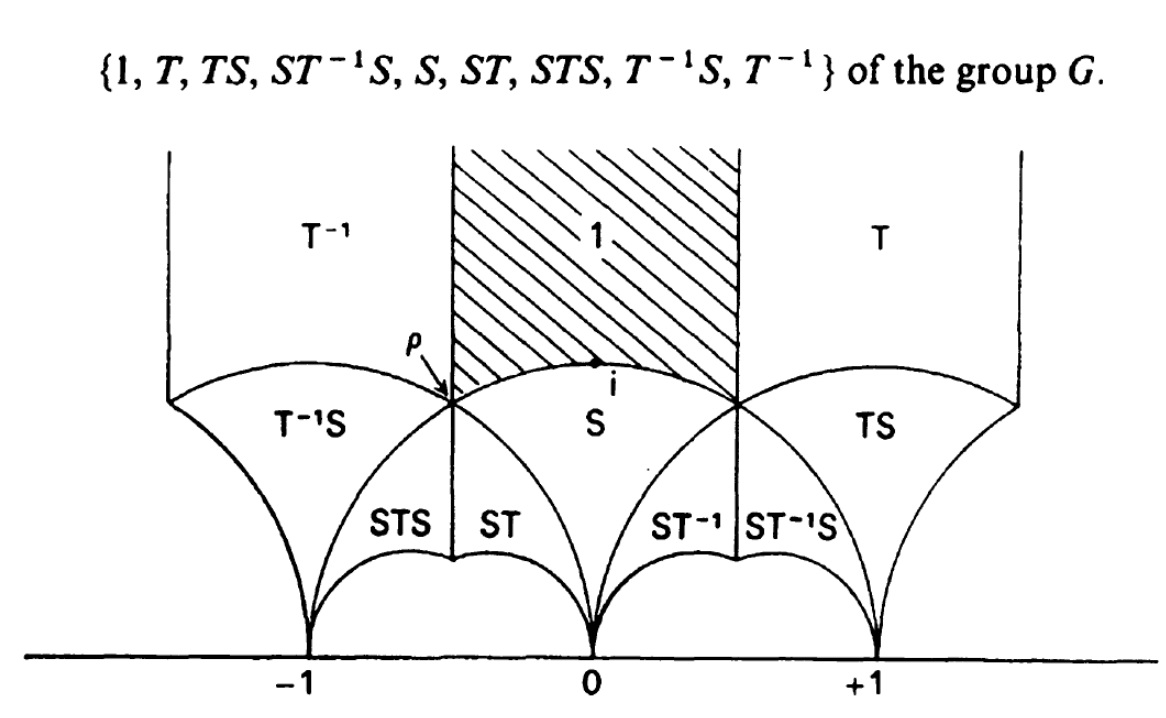
\includegraphics[width=0.5\textwidth]{FD.png}
    \caption{Above we can see a visual representation of the action of the group $G := \Gamma_0$ 
    on the striped area.}
\end{figure}



Next we can define an action of elements of $\Go$ on the Riemann sphere 
$\widehat{\C}:= \C\cup\{\infty\}$ by 
\[f(z) = \begin{bmatrix}
    a & b \\
    c & d
\end{bmatrix}(z) = \frac{az+b}{cz+d}, z\in \C\]
And we extend this to the whole Riemann sphere by defining $f(-d/c) = \infty$ 
and $f(\infty) = a/c$. These transformations are known as 
\textit{Mobius transformations}.


We define the \textit{Poincaré upper half plane} as 
\[\HH = \left\{z\in \C |\Im(z)>0\right\} \]
\exe{
    Proof that $\gamma z \in \HH$ for $\gamma\in \Gamma$ and $z\in \HH$
}

\mb 

If $f:\HH \ra \C$ is a meromorphic function which satisfies the transformation
formula 
\[f(\gamma z) = (cz+d)^kf(z), \,\,\, \gamma = 
\begin{bmatrix}
    a & b \\
    c & d
\end{bmatrix}\in \Gamma, z\in\HH\]

then we say that $f$ is \textit{weakly modular of weight $k$} for $\Gamma$ in 
particular 
\begin{eqnarray*}
    f(Sz) &= f(-1/z) = (-z)^kf(z)
    f(Tz) &= f(z+1) = f(z)
\end{eqnarray*}
The second equation tells us that $f$ has a Fourier expansion of the following form in a suitable neighborhood
of the origin, wit the origin removed:
\[f(q) = \sum_{n\in \Z}a_nq^n, \text{ with } q:= e^{2\pi i z};\]

If there exists a $m$ such that $a_n=0$ for $n<m$ we say that $f$ is \textit{meromorphic at} 
$\infty$. If in addition to this $a_n=0$ for all $n<0$, then we say that 
$f$ \textit{holomorphic at} $\infty$ 

We call $f(q)$ the \textit{Fourier expansion of $f$ at} $\infty$, or simply the  \textit{Fourier expansion of $f$.}

\df[Modular form]{}{
    Let $k$ be an integer. We say that a meromorphic function
    $f: \HH \ra \C$ is a \textit{modular form of weight $k$} for $\Gamma$
    if 
    \begin{enumerate}
        \item $f$ is weakly modular of weight $k$ for $\Gamma$
        \item $f$ is holomorphic on $\HH$
        \item $f$ is holomorphic at $\infty$
    \end{enumerate}
    We call the set of all modular forms of weight $k$ for $\Gamma$, denoted 
    $M_k(\Gamma)$ or simply $M_k$.
    
    \mb
    
    We define the value of $f$ at $\infty$ to be the limit $f(z)$ as 
    $z\ra i\infty$, and write it as $f(\infty)$. If $f$ is zero at 
    infinity then we call $f$ a \textit{cusp form}.The set of cusp forms 
    for $\Gamma$, denoted $S_k(\Gamma)$ or simply $S_k$.
}

\exe{
    Let $f \in M_k(\Gamma)$ and $g,h\in M_l(\Gamma)$ then $fg\in M_{k+l}(\Gamma)$, 
    also note that $cg\in M_l(\Gamma)$, for all $c\in \C$ and $g + h \in M_l(\Gamma)$.
    This gives the set of modular forms of weight $k$ a structure of a $\C$ vector space 
    and in addition gives the set of all modular forms on $\Gamma$, denoted $M(\Gamma)$ 
    a structure of a graded $\C$-algebra.

    \mb 

    Show a similar result for $S_k$.
}

\mb 

One other way to look at $S_k$ is that it is the kernel of the map $M_k\ra\C, f\ra f(\infty)$.

\mb 

The condition for a function to be a modular form is rather strong and one naturally 
can ask what are examples of them.

First we can note that if $f$ is a modular form of weight $k$ then 
\[f\left(\begin{bmatrix}
    -1 & 0 \\
    0 & -1
\end{bmatrix}z\right) = f(z) = (-1)^kf(z)\]
so if $k$ is an odd number then $f(z) = -f(z)$ and therefore $f$ must be the zero function. In the next section
we will see an example of a nontrivial modular form.

\section{Eisenstein series}

\prop[Eisenstein series]{}{
    Let $k$ be an even integer which is at least 4 and let $z \in \mathcal{H}.$ The function 
    \[G_k(z) = \sum_{\substack{(m,n)\in \Z^2 \\ (n,m)\neq (0,0)}} \frac{1}{(mz+n)^k}\]
    is a modular form of weight $k$ for $\Go$.
}
\pf{
    First we show that $G_k(z)$ is holomorphic on $\HH$ and at $\infty$. Fix $A,B\in\R_{+}$ 
    and then define $\D_{A,B}$ to be the set of $z\in \HH$ such that $Im(z)>A$ and $|Re(z)|<B$
    It's possible to show that there exists a $C>0$ such that for all $(\nu ,\mu )\in \R^2-\left\{0\right\} $
    and all $z\in \D_{A,B}$ then $|\nu z + \mu|>C\sup(|\nu|,|\mu|).$ 
    Note that the number of elements of $\Z^2$ such that the taxicab norm is equal to a
    given number $s\in \N_+$ is equal to $8s$. Now we have
    \[\left\lvert G_k(z)\right\rvert \leq 
    \sum_{\substack{(m,n)\in \Z^2 \\ (n,m)\neq (0,0)}}\frac{1}{|mz+n|^k}
    \leq \frac{1}{C^k}\sum_{\substack{(m,n)\in \Z^2 \\ (n,m)\neq (0,0)}}\frac{1}{\sup(n,m)^k}
    \leq \frac{1}{C^k}\sum_{\substack{(m,n)\in \Z^2 \\ (n,m)\neq (0,0)}}\frac{8s}{s^k}
    \] 
    This means that the series converges normally on $\D_{A,B}$ and therefore $G_k(z)$ 
    is a holomorphic function on $\HH$. By absolute convergence of $G_k(z)$ along with
    the bijection 
    \[(n,m)\ra(m,n+m), \,\,\, (n,m)\ra(n,-m)\] give us the relations 
    \[G_k(z+1) = G_k(z), \,\,\, G_k(-1/z) = z^kG_k(z) \] 
    for all $z\in \HH$.

    To show that $G_k(z)$ is finite at $\infty$, we will show that $G_k(z)$ approaches
    an explicit finite limit as $z\ra i\infty$. The terms of $G_k(z)$ are of the form
    $1/(mz+n)^k$, those which have $m\not= 0$ will contribute $0$ to the sum, while those
    which have $m=0$ each contribute $1/n^k$. Therefore we have
    \[\lim_{z\ra i\infty}G_k(z) = \sum_{0\neq n \in \Z} \frac{1}{n^k} = 2\zeta(k) \]
    Now let us suppose that $z$ satisfies $|z|\geq 1$ and $\Re(z) \leq 1/2$; we
}
\exe{
    Proof that there exists a $C>0$ such that for all $(\nu ,\mu )\in \R^2-\left\{0\right\} $
    and all $z\in \D_{A,B}$ then $|\nu z + \mu|>C\sup(|\nu|,|\mu|)$
}
We can see from the proof that $G_k(z)$ is not zero at infinity. 

\section{Bernoulli numbers}
\df[Bernouilli numbers]{}{
    We will define the \textit{Bernouilli numbers}, $B_n$, to be the numbers
    that satisfy the equation
    \[\frac{t}{e^t-1} = \sum_{m=0}^{\infty}B_m\frac{t^m}{m!}\]
}
\exe{
    Show that $B_1 = -1/2, B_2= 1/6, B_3 = 0$ and $B_4= -1/30$ and
    that $B_{2r+1} = 0$ for $r\geq 1$.
}

If a prime does not divide the numerator of any of the Bernoulli
numbers $B_2,B_4,\ldots,B_{p-3}$ then it is said to be a 
\textit{regular prime} and \textit{irregular} otherwise. 
Ernst Kummer proved that for all regular primes Fermat's equation
with regular prime exponents is unsolvable.

\mb 

Siegel conjectured has that about $61\%$ of primes 
are regular, which would lead to the statement that there are 
infinitely many regular primes however no one has been able to 
prove the two conjectures. Jensen however proved in a short paper in 1915 
that there are infinitely many irregular primes.

\mb

Another interesting fact about Bernoulli numbers are their relations
to the Riemann zeta function via euler's celebrated formulas

\[\zeta(2k) = (-1)^{k-1}\frac{(2\pi)^{2k}}{(2k)!}\frac{B_{2k}}{2}, \,\,\, \zeta(1-k) = -\frac{B_k}{k}\]

\section{Fourier expansions of Modular forms}

The Fourier expansions of modular forms are very arithmetically interesting, for example,
many modular forms have Fourier coefficients which are multiplicative or satisfy
recurrence relations. 


We have already seen that a modular form $f$ has a Fourier expansion in some suitable 
neighborhood of the origin. We also computed the first coefficient $a_0$ of the Fourier
expansion of $G_k(z)$. We will now exhibit the complete Fourier expansion of $G_k(z)$.
\prop[]{}{
    Let $k\geq 4$ be an even integer, and let $z\in \HH$. The modular form $G_k(z)$ has 
    Fourier expansion

    \[G_k(z)=2\zeta+2\frac{(2\pi i)}{(k-1)!}\sum_{n=1}^{\infty}\sigma_{k-1}(n)q^n,\]

    where we define $\sigma_{k}(n)$ to be the function
    \[\sigma_{k}(n):=\sum_{0<m|n}m^{k}\]
}
\pf{
    Using the identity $\frac{1}{z} + \sum_{n = 1}^{\infty} \left(
        \frac{1}{z+n} + \frac{1}{z-n}
        \right) = \frac{\pi}{\tan(\pi z)}$ we will proof the result, note that the 
        series on the left is absolutely convergent.
        The function on the right is periodic of period $1$ and therefore
        has a Fourier expansion given by 
        \[\frac{\pi}{\tan(\pi z)} = 
        \pi\frac{\cos(\pi z)}{\sin(\pi z)} =
         \pi i \frac{e^{\pi i z}+ e^{-\pi i z}}{e^{\pi i z}-e^{-\pi i z}}  = 
         -\pi i \frac{1+q}{1-q} = 2\pi i \left(\frac{1}{2} + \sum_{r=1}^{\infty}q^r\right), \]
         where $q = e^{2\pi i z}$. Using this relation and differentiating 
         the first equation $k-1$ times and divide by $(-1)^{k-1}(k-1)!$ to get 
         \[\frac{1}{z^k}\sum_{n=1}^{\infty}\left(\frac{1}{(z+n)^k}+\frac{1}{(z-n)^k}\right)\]  
         now for the Fourier expansion of $G_K(z)$
         \begin{align*}
            G_k(z) &= \frac{1}{2}\sum_{0\neq n\in\Z}\frac{1}{n^k}
         +\frac{1}{2}\sum_{\substack{(m,n)\in \Z^2 \\ m\neq 0}}\frac{1}{\sup(n,m)^k}
         = \sum_{n=1}^{\infty}\frac{1}{n^k} +\sum_{m=1}^{\infty}\sum_{n=-\infty}^{\infty}\frac{1}{(mz+n)^k}\\
            &= \zeta(k) + \frac{(2\pi i)^k}{(k-1)!}\sum_{m=1}^{\infty}\sum_{r=1}^{\infty}r^{k-1}q^{mr} \\
            &= \frac{(2\pi i)^k}{(k-1)!}\left(-\frac{B_k}{2k}+\sum_{n=1}^{\infty}\sigma_{k-1}(n)q^n\right) 
         \end{align*}
}
\exe{Show that $\frac{1}{z} + \sum_{n = 1}^{\infty} \left(
    \frac{1}{z+n} + \frac{1}{z-n}
    \right) = \frac{\pi}{\tan(\pi z)}$ 
    using the formula $\sin(x) = x^2\prod_{n=1}^{\infty}\left(1-\frac{x^2}{n^2\pi^2}\right)$ }

A standard notation for Eisenstein series is to write 
\[E_k(z):= \frac{G_k(z)}{2\zeta(k)},\]
this is called the \textit{normalized Eisenstein series of weight k}. For these modular
forms the following identities hold:
\[E_k(q) = 1 - \frac{2k}{B_k}\sum_{n=1}^{\infty}\sigma_{k-1}(n)q^n\]
\begin{align*}
    E_4(q) &= 1 + 240\sum_{n=1}^{\infty}\sigma_3(n)q^n \\
    E_6(q) &= 1 -504\sum_{n=1}^{\infty}\sigma_5(n)q^n \\
    E_8(q) &= 1 + 480\sum_{n=1}^{\infty}\sigma_7(n)q^n \\
    E_{10}(q) &= 1 - 264\sum_{n=1}^{\infty}\sigma_{9}(n)q^n \\
    E_{12}(q) &= 1 + \frac{65520}{691}\sum_{n=1}^{\infty}\sigma_{11}(n)q^n \\
    E_{14}(q) &= 1 + 240\sum_{n=1}^{\infty}\sigma_{13}(n)q^n    
\end{align*}

We saw that if $k=2$ then the sum in $G_2$ does not converge but what we can do to give 
$E_2$ some meaning is to define by following the pattern and defining it by its Fourier expansion 

\prop[]{}{
    There is a holomorphic function $E_2$ which has Fourier expansion at $\infty$
    \[E_2(q) = 1-24\sum_{n=1}^{\infty}\sigma_1(n)q^n,\]
    which satisfies the following transformation formula 
    \[E_2\left(\frac{az+b}{cz+d}\right)  = (cz+d)^2E_2(z) + \frac{12}{2\pi i}c(cz+d)\]

}

\section{Ramanujan $\Delta$ function}

In the early $20^{th}$ century Srinvasa Ramanujan studied the explicit Fourier expansions of considerations 
well-known modular forms, such as the $\Delta$ function, given by 

\[\Delta(z) := q\prod_{n=1}^{\infty}(1-q^n)^{24} = \sum_{n=1}^{\infty}\tau(q)q^n,\]

where $q = e^{2\pi i z}$. We can expand the product in the definition to get 

\[\Delta(z) = q - 24q^2+ 252q^3 - 1472q^4 + 4830q^5 - 6048q^6 - 16744q^8- 113643q^9 + \ldots\]

\mb 

Ramanujan observed in 1915 that $\tau(n)$ is multiplicative, i.e. $\tau(mn) = \tau(m)\tau(n)$
for coprime $n$ and $m$. 

\prop[]{}{
    The function $\Delta(z)$ is a cusp form of weight 12.
}
\pf{
    Since $\Delta(z) \neq 0,$ we can consider its logarithmic derivative. We find 
    \[\frac{1}{2\pi i}\frac{d}{dz}log(\Delta(z)) = 
    \frac{1}{2\pi i}\frac{d}{dz}\left(q\prod_{n=1}^{\infty}(1-q^n)^{24}\right) =
    \frac{1}{2\pi i}\frac{d}{dz}\left(log(q) + 24\sum_{n=1}^{\infty}log(1-q^n)\right) \]

    Since $q = e^{2\pi i z}$ we have $\frac{1}{2\pi i}\frac{d}{dz}$ and therefore

    \[\frac{1}{2\pi i}\frac{d}{dz}log(\Delta(z)) =
     1 - 24\sum_{n=1}^{\infty}n\frac{q^n}{1-q^n} =
     1 - 24\sum_{n=1}^{\infty}n\sum_{d=1}^{\infty}q^{dn} = 
     1 - 24\sum_{n=1}^{\infty}\sigma_1(n)q^n = E_2(z).
    \]

    Now we have already seen that 
    \[E_2\left(\frac{az+b}{cz+d}\right) = (cz+d)^2E_2(z) + \frac{12}{2\pi i}c(cz+d).\]

    Combining the equations above and using the fact that 
    
    \[\frac{d}{dz}\left(\frac{az+b}{cz+d}\right) = \frac{1}{(cz+d)^2}\]

    for $\gamma =\twobytwo{a}{b}{c}{d} \in \Gamma,$ we deduce that 

    \[\frac{1}{2\pi i }\frac{d}{dz} log\left(\frac{\Delta\left(\frac{az+b}{cz+d}\right)}{(cz+d)^{12}\Delta(z)}\right)
    = \frac{1}{(cz+d)^2}E_2\left(\frac{az+b}{cz+d}\right) - \frac{12}{2\pi i} \frac{c}{cz+d} - E_2(z) = 0.\]

    In other words, $log(\Delta\left(\frac{az+b}{cz+d}\right)) = log(s(\gamma))log((cz+d)^12\Delta(z))$, where $s(\gamma)$ is a non zero constant that
    depends only on $\gamma$ that is 
    \[\Delta\left(\frac{az+b}{cz+d}\right) = s(z)(cz+d)^12\Delta(z)\]

    we want to show that $s(\gamma) = 1$ for all $\gamma\in \Gamma$.

    \mb

    First note that for $\gamma_1 = \twobytwo{a_1}{b_1}{c_1}{d_1}$ and 
    $\gamma_2 = \twobytwo{a_2}{b_2}{c_2}{d_2}$ with $\gamma_3:= \gamma_1\gamma_2 = 
    \twobytwo{a_3}{b_3}{c_3}{d_3}$ we have  
    
    \[s(\gamma_1)s(\gamma_2)\Delta(z) = s(\gamma_1)\Delta\left(\gamma_2z\right)(c_2z+d_2)^{-12}=
     \Delta(\gamma_1\gamma_2z)(c_3z+d_3)^{-12}= s(\gamma_1\gamma_2)\Delta(z).\]

     Therefore $s:\Gamma \ra \C$ is a homomorphism so we just need to prove that $s(T) = s(S)= 1$.

     \mb

     By definition we have $\Delta(Tz) = \Delta(z)$ so $s(T) = 1$ and to show that $s(S) = 1$ put 
     $z= i$ in the equation $z^{-12}\Delta(\frac{-1}{z}) = s(S)\Delta(z).$
}  


\section{Dimension of $M_k(\Gamma)$ and $S_k(\Gamma)$}
We have already seen that $M_k$ and $S_k$ have a structure of a $\C$ vector space. In this section we will look at the dimension of the $\C$ vector spaces of modular forms of 
weight $k$ and cusp forms of weight $k$.

\mb 

First let us define the order of a meromorphic function $f:\HH \ra \C$ at a given point $x\in \HH$,
 denoted $v_x(f)$, as the integer $n$ such that $f(z)/(z-x)^n$ is holomorphic and non null. We can 
 furthermore define $v_\infty(f)$ as the order of $f$ in the Fourier expansion at $q=0$. This integer 
 is necessarily positive since it counts the number of poles of $f$ at $x$.
 
\mb 

When $f$ is a modular form of weight $k$ then the identity
\[f(z) = (cz+d)^{-k}f(\frac{az+b}{cz+d})\]
shows us that $v_x(f) = v_{\gamma x}(f)$ if $\gamma \in \Gamma$. Thus we can define $v_{\bar{x}}(f)$
where $\bar{x}$ is in the quotient $\HH/\Gamma$ because $v_x(f)$ does not depend on 
the representative of $x$ in $\HH/\Gamma$.


\mb

now for a lemma that is very useful when studying the dimension of $M_k(\Gamma)$ will be stated without 
proof but the reader is encouraged to see \cite{Serre:1993} for a complete proof.

\thm[The $k-12$ lemma]{}{
Let $f$ be a modular form of weight $k$ that is not the zero function, then we have the equation:
\[v_\infty(f)+ \frac{1}{2}v_i(f) + \frac{1}{3}v_\rho(f) + \sum_{x\in\HH/G} v_x(f) = \frac{k}{12}\]
}

Using this lemma we proof the proposition
\prop[Formulae for the full modular group]{}{
    Let $k$ be an integer. Then 
    \begin{itemize}
        \item $M_0(\Gamma) = \C$
        \item $M_2(\Gamma)=0$, and if $k<0$ or if $k$ is odd then $M_k(\Gamma)=0$
        \item If $k\in \{4,6,8,10,14\}$, then $M_k(\Gamma)=\C E_k$
        \item If $k<12$ or $k=14$ then $S_k(\Gamma)=0,S_{12}(\Gamma)=\C\Delta$ and if $k\geq 16$ then $S_k(\Gamma)=\Delta M_{k-12}(\Gamma)$
        \item If $k\geq 4$ then $M_k(\Gamma)=S_k(\Gamma)\oplus \C E_k$
    \end{itemize}
}
\pf{
    i) We know that the constant functions are elements of $M_0$ and we want to show the reverse.
    Let $f\in M_0$ be an arbitrary modular form of weight $0$ and let $z \in \C$ be any element in the image
    of $f$. Then $f(z) - c \in M_0$ has a zero in $\HH$, i.e. one of the terms in the equation in the $k-12$ lemma
    is strictly positive. Since the right-hand side is $0$, this can only happen if $f(z) - c$ is the zero function,
    i.e. $f$ is constant.
    
    \mb
    
    ii) We already saw that $M_k = 0$ if k is odd. if $k = 2$ or $k < 0$ then $k/12$ is negative or $1/6$, which has no positive solutions on the left-hand side
    
    \mb
    
    iii) If $k\in \{4,6,8,10,14\}$, then there is only one possible way of choosing the $v_x(f)$ in the $k-12$ lemma is:
    \begin{itemize}
        \item $k = 4$ : $v_\rho(f) = 1$ and all other $v_x(f) = 0$.
        \item $k = 6$ : $v_i(f) = 1$ and all other $v_x(f) = 0$.
        \item $k = 8$ : $v_\rho(f) = 2$ and all other $v_x(f) = 0$.
        \item $k = 10$ : $v_\rho(f) = v_i(f) = 1$ and all other $v_x(f) = 0$.
        \item $k = 14$ : $v_\rho(f) = 2, v_i(f) = 1$ and all other $v_x(f) = 0$.
    \end{itemize}
    
    \mb

    iv) If $f \in S_k$ we have $v_\infty(f) > 0$, which is not possible by the $k-12$ lemma for $k < 12$ or $k = 14$.

    \mb

    v) We know that $v_\infty(\Delta) = 1$ and by the $k-12$ lemma this can be the only zero of $\Delta$.
    Therefore for any $f \in S_k$ the function $f\Delta$ is a modular form of weight $k - 12.$
    
    \mb 

    vi) If $f\in M_k$ is not a cusp form then its Fourier expansion at $\infty$ has a non zero constant term $c$.   
    We note that $f - c E_k$ ia a modular form of weight $k$ and has a zero constant term in its Fourier expansion, 
    i.e. $M_k = \C E_2 \bigoplus S_k$   
}

\thm[Dimenton of $M_k(\Gamma)$ and $S_k(\Gamma)$]{}{
Let $K$ be an even positive integer. Then
\[ 
\dim M_k(\Go)= \left\{
\begin{array}{ll}
    \lfloor\frac{k}{12}\rfloor + 1, \text{ if } k\not\equiv 2 \mod 12 \\
    \lfloor\frac{k}{12}\rfloor, \text{ if } k\equiv 2 \mod 12 
\end{array} 
\right. 
\]    
and
\[ 
\dim S_k(\Go)= \left\{
\begin{array}{ll}
    \lfloor\frac{k}{12}\rfloor, \text{ if } k\not\equiv 2 \mod 12 \\
    \lfloor\frac{k}{12}\rfloor - 1, \text{ if } k\equiv 2 \mod 12 
\end{array} \right. 
\]    
}
\pf{
    We will proceed by induction. We already know the formulas to be true for $k\leq 14$. 
    Now by the 5th point of the proposision above we know that the dimention of $S_k$ is one
    less than the dimension of $M_k$. It suffices to prove the theorem for $M_k$.

    \mb 

    Assume we have proved the formula for $k$ and now we consider the dimension of $M_{k+12}$. 
    From the preceding proposition we see that 
    \[M_{k+12} = \C E_{k+12}\bigoplus \S_{k+12} = \C E_{k+12} \bigoplus \Delta M_k,\]
    and now we use the induction hypothesis to get the result.
}

Let's now show that it can be equivalently defined as \[\Delta=\frac{E_4^3-E_6^2}{1728}\].

\mb

We know that $\Delta$ is a modular form of weight $12$. Also by the graded $\C$ algebra structure
of modular forms we have that $E_4^3,E_6^2\in M_12$. Now the constant term of $E_4^3$ and $E_6^2$ 
are both equal to one and thus $E_4^3-E_6^2 \in S_12$. But we have seen that the dimension of 
$S_12$ as a $\C$ vector space is equal to one. We can now see that $E_4^3-E_6^2 = C\Delta$. Now 
we can write 
\begin{align*}
    E_4^3(q) &= (1+240q+O(q^2))^3 = 1 + 720q + O(q^2) \\
    E_6^2(q) &= (1-504q+O(q^2))^2 = 1 -1008q + O(q^2) \\
    E_4^3-E_6^2 &= 1728q + O(q^2)\\
    \Delta(q) &= q + O(q^2)
\end{align*}

By comparing the coefficients at $q$ we can deduce that $C= 1728$ proving the formula.

\section*{Conclusion}
\begin{quotation}
    Mathematics is not a spectator sport.
    \mb
    -George Polya. 
\end{quotation}

\exe{
    Proof the following relations:
    \begin{align*}
        \sigma_7(n) &= \sigma_3(n)+\sum_{i=1}^{n-1}\sigma_3(i)\sigma_3(n-i) \\
        11\sigma_9(n) &= 21\sigma_5(n)-10\sigma_3(n)+5040\sum_{i=1}^{n-i}\sigma_3(i)\sigma_5(n-i) \\
        \sigma_{13}(n) &= 21\sigma_5(n)-20\sigma_7(n)+10080\sum_{i=1}^{n-i}\sigma_5(i)\sigma_7(n-i) \\
        \tau(n) &\equiv \sigma_{11}(n) \mod 691    
    \end{align*}
}
\exe{
    Let $\Delta = \frac{1}{1728}(E_4^3-E_6^2) = \sum_{n=1}^{\infty}\tau(n)q^n$ and $D$ 
    be the opperator $D = \frac{1}{2\pi i}\frac{d}{d\tau} = q\frac{d}{dq}$
    \begin{enumerate}
        \item Show that the fonction $H = 4E_4D(E_6)-6E_6D(E_4)$ is a modular form 
        of weight $12$.
        \item Deduce that 
        \[\tau(n) = \frac{n}{12}(5\sigma_3(n)+7\sigma_5(n))+\sum_{1\leq m\leq n}(2n-5m)\sigma_3(m)\sigma_5(n-m)\]
        \item Conclude that 
        \[\tau(n)\equiv n\sigma_5(n)\equiv \sigma_1(n) \text{ mod } 5,\]
        \[\tau(n)\equiv n\sigma_3(n) \text{ mod } 7.\]
    \end{enumerate}
}


The reader is encouraged to look through the Bibliography for a more thorough look at the field of
modular forms, in particular \cite{Kilford:2008} for as an Introduction, \cite{Serre:1993} for a elegant
concise view of the basics, \cite{Ramanujan:2012} for 
more interesting congruences and \cite{Ranestad:2008} for various applications of modular forms.